% !TEX root = Dokumentation.tex


\newpage
\section{Anhang}
 
\begin{itemize}
  \item[\textbf{I}] Technologierecherche (26 Seiten)
  \item[\textbf{II}] Aufgabenstellung (8 Seiten)
  \item[\textbf{III}] Anforderungsliste (5 Seiten)
  \item[\textbf{IV}] Morphologischer Kasten (44 Seiten)
\end{itemize}
 
\includepdf[pages={-}]{../Technologierecherche/Technologierecherche.pdf}
\includepdf[pages={-}]{./Images/AufgabenstellungV3.pdf}
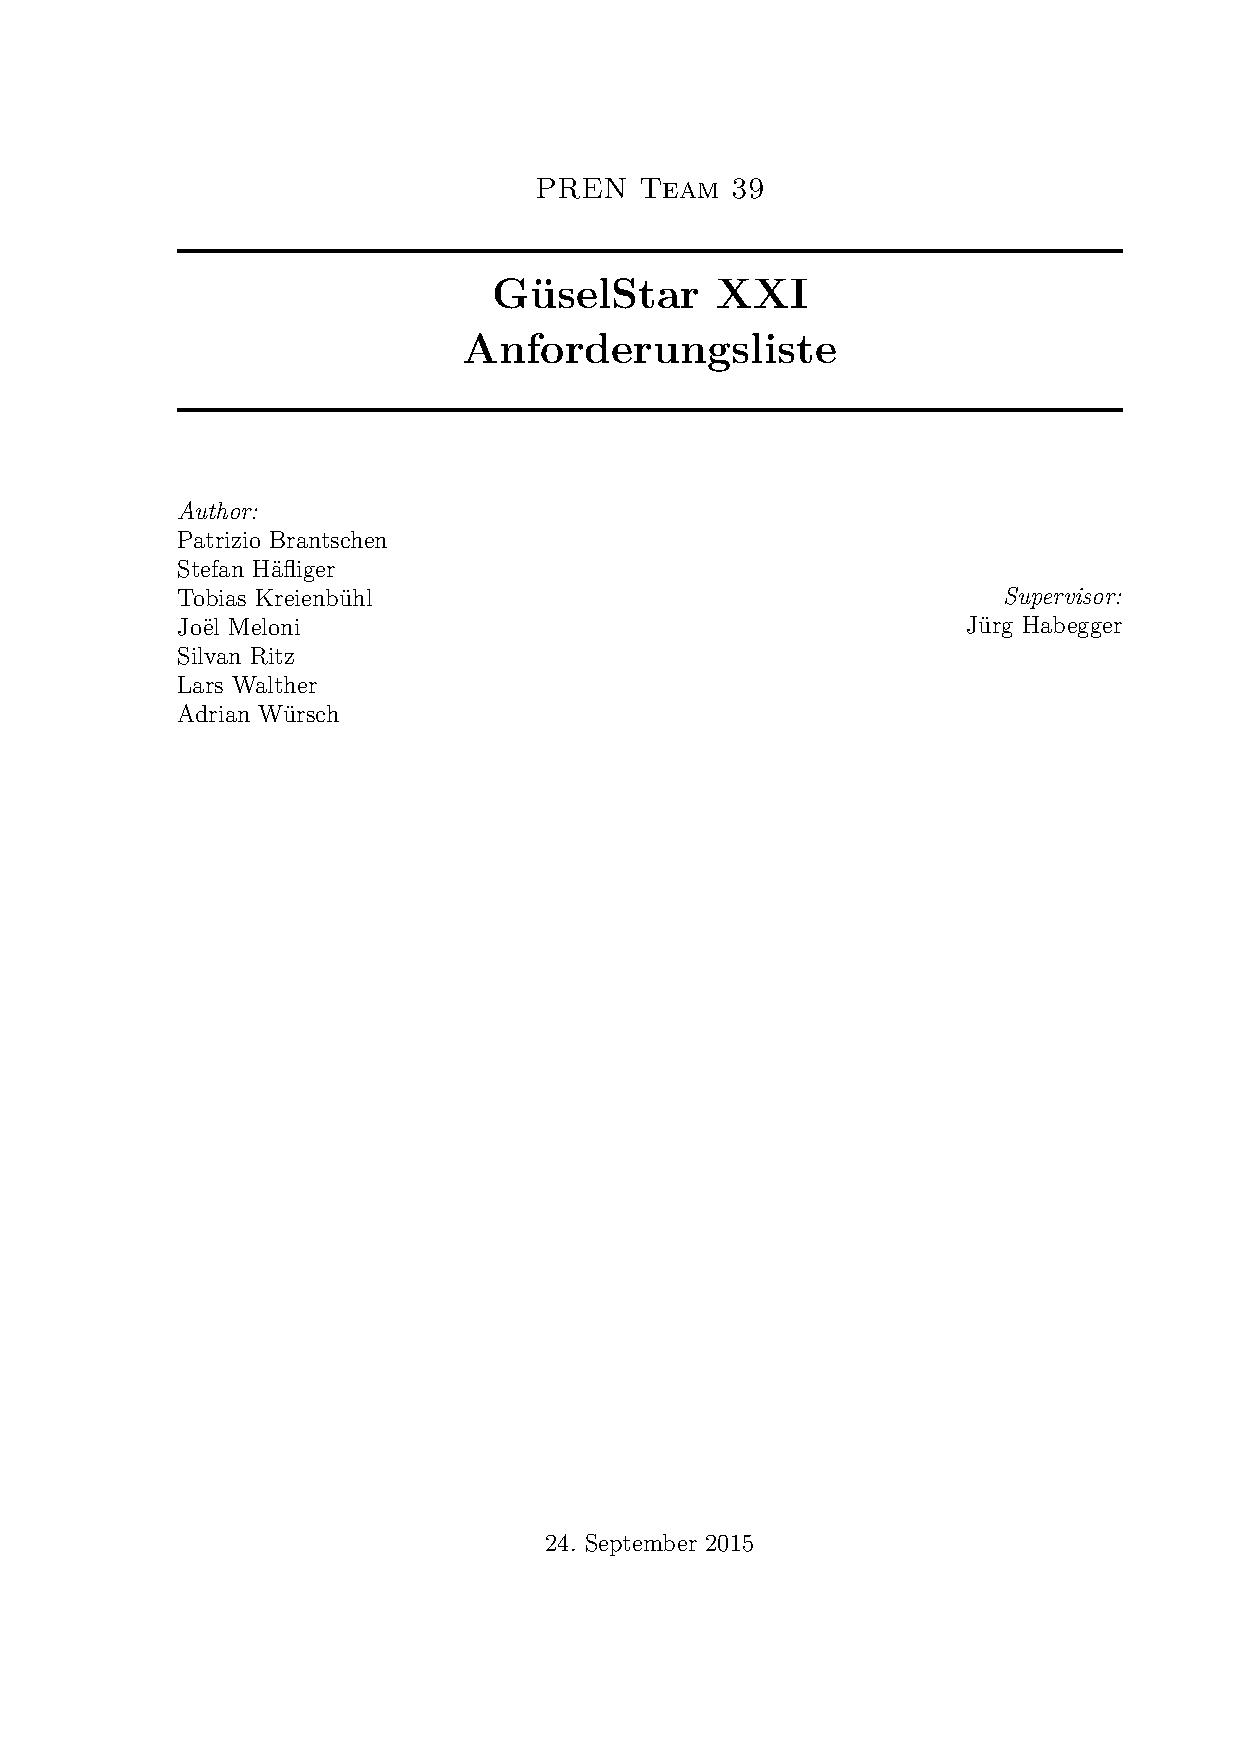
\includepdf[pages={-}]{../Anforderungsliste/Anforderungsliste.pdf}
\includepdf[pages={-}]{../MorphologischerKasten/morphkasten.pdf}



